
Power is becoming a major financial and environmental concern, restricting the compute
capacity of High Performance Computing (HPC) systems.  Today's most power efficient
supercomputer operates at 14.1GFLOPS/W~\cite{Green500:2017}, but even if we had a system
able to operate at the 50GFLOPS/W rate, which is the limit that some funding agencies have
set up for building an exascale machine, the full system would consume several tens of
MWatts of power, which constitutes a large economic burden.  Consequently, a report from
the US Department of Energy (DOE)~\cite{ASCAC:tech:2014} identifies energy efficiency as
one of the top ten research challenges on the road to exascale.  For similar reasons, the
European Union has set up an HPC program % is also concerned and focused on building
low-power systems based on mobile technology~\cite{Rajovic2013}.
\par
An emerging design practice for HPC systems, known as 
\textit{overprovisioning}~\cite{patki:2013:eho:2464996.2465009}, is to have more nodes
than the maximum power budget could feed if run at peak capacity, in contrast to
traditional approaches, which are focused in having enough power even when all nodes run
at their peak. Overprovisioning is driven by the observation that most applications in 
practice never reach peak power and hence do not fully utilize the available power envelope. 
In such overprovisioned systems, we can lower the average power provisioned to each node, 
allowing us to power more nodes within the same power budget. This approach is made possible 
by recent developments in hardware design that enable power management and power capping from 
user space, as this is necessary to efficiently manage power as a limited and shared resource. 
As an alternative to restricting power to nodes, we can choose to only operate fewer but at 
full power. Their total power consumption should not exceed that of the total power budget. 
This second approach restricts the available parallelism in the system, but allows for faster 
execution and does not force us to deal with any complications related slower then expected 
execution of the system’s workload. Which approach is preferable (or a combination of both) 
should depend on system and workload characteristics. For example, whether the workload would 
benefit from extra processing units or limitations in the completion time set by the user
or administrator.
\par
Workloads at the HPC system level  are managed by job schedulers that allocate resources
to dispatched jobs.  Such jobs can run on distributed memory scenarios and, in this
context, MPI~\cite{Nagle:2005:MCR:1239662.1239666} is the most common approach to handle
distributed memory communications.  It is usually coupled with a shared memory programming
model, like OpenMP~\cite{openmp13} or similar~\cite{10.1007/978-3-540-85261-2_5}.
Either across nodes or within a shared-memory node, both job and runtime schedulers deal
with the resource allocation problem, albeit at different levels, offering opportunities
to manage power consumption.  Indeed, examples of power-aware systems  that offer
solutions either at the job scheduling
\cite{Gholkar:2016:PTH:2967938.2967961,7515666,Ellsworth:2015:DPS:2807591.2807643,Etinski2012615}
or at runtime system  \cite{Gholkar:2016:PTH:2967938.2967961,
Chasapis:2016:RMM:2925426.2926279,Totoni:tech:2014,Teodorescu:2008:VAS:1381306.1382152,Inadomi:2015:AMI:2807591.2807638}
levels already exist in the literature.
\par
Manufacturing variability or process variation refers to the power and frequency
heterogeneity observed across chips implementing the exact same architecture as a
consequence of uncontrollable material differences in the manufacturing
process~\cite{Rountree:2012:BDF:2357488.2357648}.  In order to provide homogeneous
performance, chips of the same architecture must hide frequency variability, which can
only be achieved via variations in their power consumption.  However, in a power
constrained environment where all chips need to operate under a certain power cap, this
frequency variability can no longer be hidden~\cite{Rountree:2012:BDF:2357488.2357648},
leading to heterogeneous performance.  As a result, a theoretically homogeneous system
turns into a heterogeneous one with performance variations of up to
64\%~\cite{Inadomi:2015:AMI:2807591.2807638}.  While ignoring this manufacturing
variability leads to performance and energy inefficiencies, there are opportunities for
achieving improvements at the power budgeting or parallel runtime system levels when
variability is properly
managed~\cite{Chasapis:2016:RMM:2925426.2926279,Teodorescu:2008:VAS:1381306.1382152,Inadomi:2015:AMI:2807591.2807638,Gholkar:2016:PTH:2967938.2967961,Totoni:tech:2014}.

\begin{figure}
	\centering
	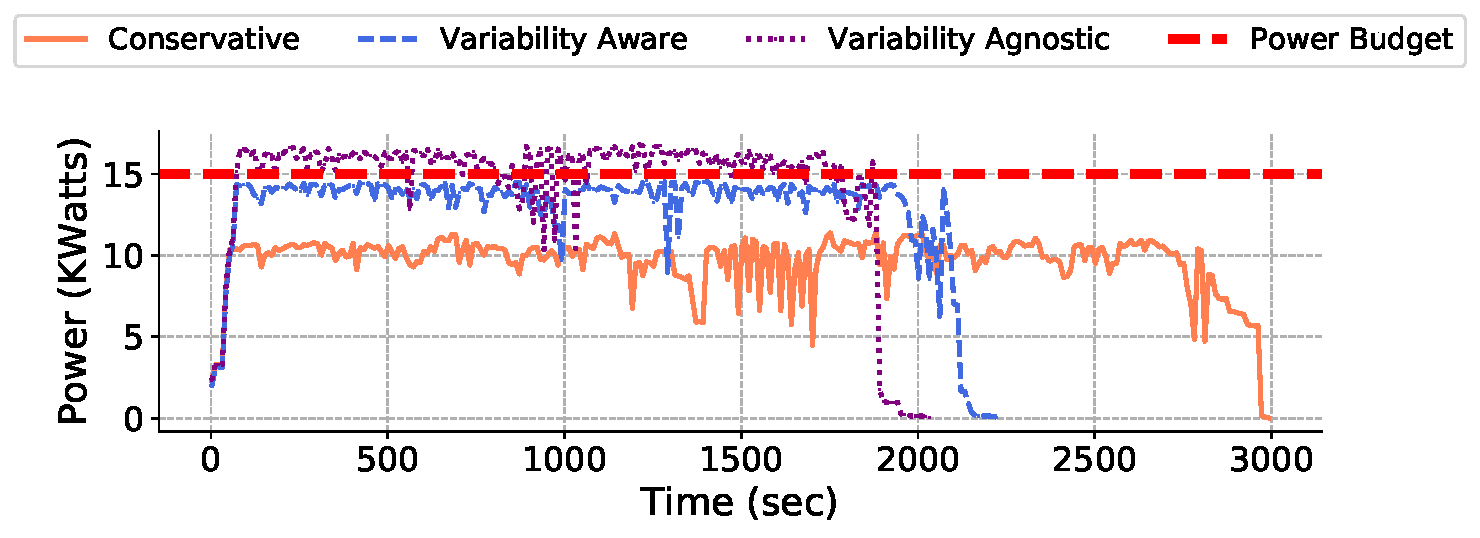
\includegraphics[width=\columnwidth]{power_aware_job_scheduling/figures/motivation}
	\caption{Total power consumption trace for Conservative, Variability agnostic and 
		Variability aware scheduling policies, when running the same workload.  
		Considering socket variability maximizes performance 
		and meets the power budget.}
	\label{fig:motivation}
	%\vspace{-.3cm}
\end{figure}

\par
This thesis goes beyond the state-of-the-art by proposing job scheduling policies driven by
variability-aware power prediction models.  We consider two different approaches to
predicting manufacturing variability.  The first model assumes that all applications
are affected the same way by manufacturing variability.  This assumption is not correct, as 
demonstrated in Section \ref{sec:model_validation}. The second model offers a more robust
approach, where the model uses a training set of applications to identify how different application
behavior is impacted by manufacturing variability.
We extend power-aware scheduling and power
prediction models to deal with manufacturing variabity,  producing two novel variability-
and power-aware job scheduling policies.  The goal of these policies is to maximize the
utilization of the cluster without exceeding the available power budget and without
restricting per socket power consumption.  Instead, by using the power prediction, the
policies can find the maximum number of concurrent jobs that can run within the power
budget.  This offers an alternative to per node power capping, which in combination with
manufacturing variability, would create an heterogeneous cluster.  Current workload
managers do not account for this type of heterogeneity.   
We consider the power consumption of the CPU,
since it accounts for more than 50\% \cite{ShuaiwenSong:2009:EPA:1572226.1572228} of the
total node's power consumption.  Our Policies rely on two different models and leverage
their power requirement predictions of individual parallel jobs to make scheduling
decisions that maximize performance while reducing energy consumption.  Many different
variability-agnostic power and energy prediction models have been proposed
~\cite{Bircher:2012:CSP:2196827.2196987,Bertran:2012:SEC:2457472.2457499,Bertran:2010:DRP:1810085.1810108,Goel:2010:PSP:1909624.1909734,Isci:2003:RPM:956417.956567}
	and are often employed to manage power distribution on clusters to mitigate the effects of
manufacturing variability
~\cite{Chasapis:2016:RMM:2925426.2926279,Inadomi:2015:AMI:2807591.2807638,Gholkar:2016:PTH:2967938.2967961,Ellsworth:2015:DPS:2807591.2807643,Bailey:2015:FLP:2807591.2807637,Teodorescu:2008:VAS:1381306.1382152,Totoni:tech:2014}.
\par
As a motivation we show Figure~\ref{fig:motivation}, where three different scheduling
policies are compared.  The Conservative simply considers that all jobs consume the same
power on all sockets.  The Variability agnostic predicts accurately the power consumption
of individual jobs, but does not consider socket variability.  On the contrary, the
Variability aware policy does also consider socket variability, making a different
prediction per socket.  As displayed in Figure~\ref{fig:motivation}, the Conservative policy is
the one providing the worse performance. The Variability agnostic improves performance by
making more accurate predictions but fails to account for the more power consuming
sockets, exceeding the 15KWatts power budget.  Finally,  the Variability aware policy
manages to improve performance, while respecting the power budget.  
Figure~\ref{fig:motivation} illustrates how accounting for manufacturing variability while scheduling parallel jobs provides performance benefits.
Section~\ref{sec:experimental_setup} describes the experimental setup we consider to generate Figure~\ref{fig:motivation}.

%Precise knowledge of
%the power consumption of individual jobs on all available sockets, while considering their
%avialability can have a significant impact in performance and optimize power utilization.
\par
This thesis shows how variability-aware power prediction models can be effectively used to
guide job scheduling policies and bring significant benefits with respect to the
variability-agnostic ones.
In particular, this thesis makes the following contributions beyond the state-of-the-art:
\begin{itemize} 

	\item Two new variability-aware power prediction models. 
				Both models use Performance Monitoring Counters (PMC) to
				predict an application's 
				power consumption on a specific socket.
				PMCs are used to measure the activity of individual architectural components while 
				the targeted application is running and a linear model is then used to find their 
				contribution to power consumption.
				The first model assumes power variability to impact all applications equally.  
				It uses a single benchmark to measure the power consumption variability across 
				sockets and apply it to the variability agnostic PMC-based model.  
				The second model extends the PMC-based approach to take power consumption 
				variability into account, as part of the model.  It trains the model for each 
				individual socket, using a reduced set of benchmarks.

	\item Two power- and variability-aware job scheduling policies that optimize job 
				turnaround time and energy efficiency while respecting a system-wide power budget.  
				Unlike previous work that does not consider variability during job scheduling 
				decisions~\cite{Inadomi:2015:AMI:2807591.2807638,Teodorescu:2008:VAS:1381306.1382152,Ellsworth:2015:DPS:2807591.2807643,Gholkar:2016:PTH:2967938.2967961}, 
				our policies use variability-aware predicton model to guide scheduling.

	\item A complete evaluation of the two variability-aware policies via a discrete event 
				simulator.  We implement additional scheduling policies for our evaluation, which 
				represent traditional and state-of-the-art  practices used in today's HPC systems.  
				Our evaluation demonstrates how variability-aware policies achieve energy savings 
				up to \MaxEnergy\% and job turnaround time reductions up to \MaxJTT\%, considering 
				different power budgets and two workload traffic scenarios (bursty and heavy).
\end{itemize}    	

The remainder of this Chapter is organized as follows.
Section~\ref{sec:variability_prediction} presents the two variability-aware power
prediction models.  Section~\ref{sec:job_sched_scheduling} introduces the variability and
power-aware scheduling policies we propose.  A validation of the models and evaluation of
our job scheduling policies are presented in Section~\ref{sec:job_scheduling_results}
and, finally, Section~\ref{sec:job_sched_conclusions} provides summarizes the
ideas and results presented in the Chapter.


\begin{table}
	\centering
	\caption{Architectural component activity ratios formulas for Intel \ARCH~Architecture,
inferred from Intel's 64 and IA-32 Architectures Software Developer's Manual
\cite{fquesnel:progguide:intel10}}
	\label{tab:comp_formulas}
	\begin{tabular}{ | c | m{10cm} | } 
		\hline
		\textbf{Power Component} & \textbf{Component Activity Formula} \\ 
		\hline
		\hline
		Fetch & UOPS\_RETIRED.ALL / CPU\_CLK\_UNHALTED.THREAD\_P \\ 
		\hline
		Branch Prediction Unit & BR\_INSTR\_RETIRED.ALL\_BRANCHES / CPU\_CLK\_UNHALTED.THREAD\_P \\ 
		\hline
		Arithmetic \& Logic Unit & (UOPS\_DISPATCHED\_PORT.PORT\_0 + UOPS\_DISPATCHED\_PORT.PORT\_1 + UOPS\_DISPATCHED\_PORT.PORT\_5) / CPU\_CLK\_UNHALTED.THREAD\_P \\ 
		\hline
		Floating Point & FP\_COMP\_OPS\_EXE.X87 / \newline CPU\_CLK\_UNHALTED.THREAD\_P \\ 
		\hline
		L1 cache & L1D\_ALL.REF / CPU\_CLK\_UNHALTED.THREAD\_P \\ 
		\hline 
		L2 cache & (L2\_RQSTS.ALL\_RFO + \newline L2\_RQSTS.ALL\_DEMAND\_DATA\_RD) / \newline CPU\_CLK\_UNHALTED.THREAD\_P \\ 
		\hline	
		L3 cache & LLC.References / CPU\_CLK\_UNHALTED.THREAD\_P \\ 
		\hline
		Memory & LLC.Misses / CPU\_CLK\_UNHALTED.THREAD\_P \\ 
		\hline
	\end{tabular}
%	\vspace{-.5cm}
\end{table}

